\documentclass[11pt,english,french]{scrreprt}
\usepackage{lmodern}
\usepackage{babel}
\renewcommand{\familydefault}{\rmdefault}
\usepackage[T1]{fontenc}
\usepackage{ucs}
\usepackage[utf8x]{inputenc}
\usepackage[a4paper]{geometry}
\geometry{verbose,tmargin=3cm,bmargin=3cm,lmargin=2cm,rmargin=2cm,headheight=2cm,footskip=2cm}
\setlength{\parskip}{\smallskipamount}
\setlength{\parindent}{0pt}

\usepackage{amsthm}
\usepackage{booktabs}
\usepackage{amsmath}
\usepackage[unicode=true, pdfusetitle,
 bookmarks=true,bookmarksnumbered=false,bookmarksopen=false,
 breaklinks=false,pdfborder={0 0 1},backref=false,colorlinks=false]
 {hyperref}

\makeatletter
\usepackage{colortbl}
\usepackage{color}
\usepackage[dvipsnames]{xcolor}
\usepackage{listings}
\usepackage[calcwidth]{titlesec}
\usepackage{fix-cm}
\usepackage{multicol}
\usepackage{wrapfig}
\usepackage{graphicx}
\usepackage{verbatim}
\usepackage{moreverb}
\usepackage{url}

\theoremstyle{remark}
  \newtheorem*{rem*}{Remarque}
\theoremstyle{definition}
  \newtheorem*{defi}{Définition}
  \newtheorem{ques}{Question}[section]
  \newtheorem{ques*}{Question}[subsection]

\definecolor{MyDarkBlue}{rgb}{0,0.08,0.45}

\lstset{language=C,
	 	basicstyle=\small\ttfamily,
		keywordstyle=\small\ttfamily,
		identifierstyle=,
		commentstyle=\textcolor{OliveGreen},
		columns=fullflexible,
		stringstyle=\small\ttfamily,
		showstringspaces=false,numberstyle=\tiny, breaklines=false, tabsize=4}

\titleformat{\section}[hang]{\sffamily\bfseries}
 {\Large\thesection}{12pt}{\Large}[{\titlerule[0.5pt]}]

\def\thickhrulefill{\leavevmode \leaders \hrule height 1pt\hfill \kern \z@}
\renewcommand{\maketitle}{\begingroup%
    \let\footnotesize\small
    \let\footnoterule\relax
    \parindent \z@
    \reset@font
    \begin{flushleft}
      \huge \sffamily \bfseries\color{orange} \@title
    \end{flushleft}
    \hrule height 1pt
    \begin{flushright}
      \large\sffamily\color{MyDarkBlue}\@author
    \end{flushright}
  \endgroup%
  \setcounter{footnote}{0}%
}

\AtBeginDocument{
  \def\labelitemi{\normalfont\bfseries{--}}
}

\makeatletter
\renewcommand\thesection{\arabic{section}}
\@addtoreset{section}{chapter}
\makeatother

\makeatother
\begin{document}
	
\title{LI310 - TME 2\\
Analyses de trames -- outil WireShark}
\author{Benjamin BARON}

\maketitle

\section{Analyse manuelle de trames} % (fold)


\begin{figure}[h!]
	\center
	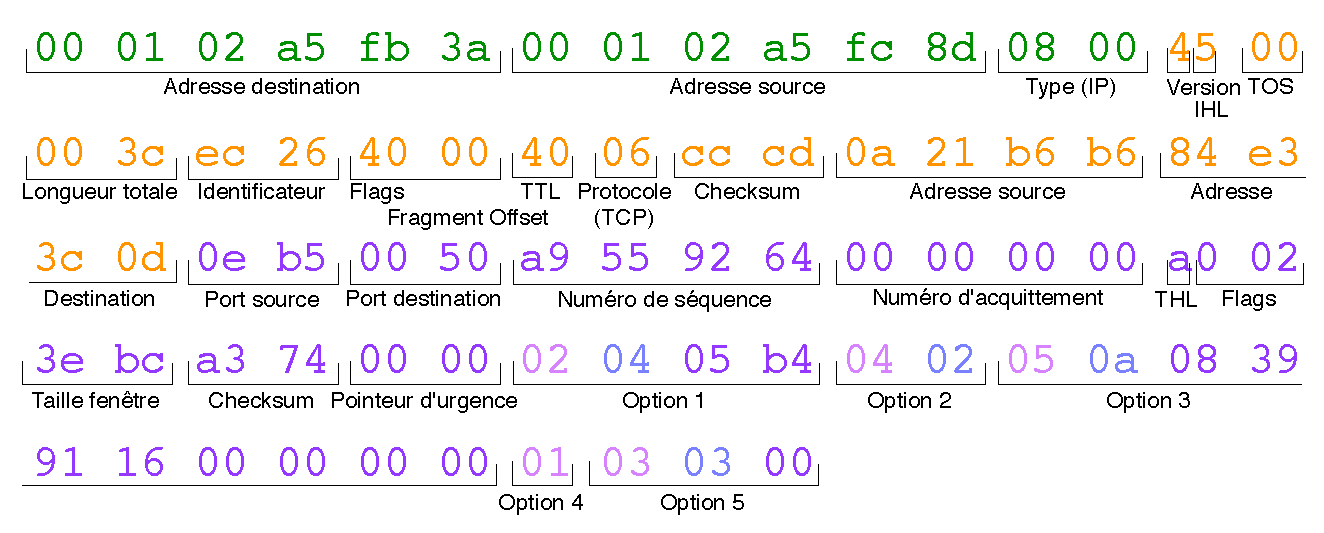
\includegraphics[scale=.7]{graphes/trame-ethernet}
	\caption{Trame ethernet décomposée}
\end{figure}

\begin{ques}
	Informations de niveau liaison :\begin{itemize}
		\item Adresse destination : \lstinline!00:01:02:a5:fb:3a!
		\item Adresse source : \lstinline!00:01:02:a5:fc:8d!
		\item Type de la trame : \lstinline!0x0800! -- DoD Internet (IP)
	\end{itemize}
\end{ques}

\begin{ques}
	Information de niveau réseau :\begin{itemize}
		\item \lstinline!Version : 0x4! -- Utilisation de IPv4
		\item \lstinline!IHL : 0x5! -- $5 \times 4 = 20$ octets $\Rightarrow$ délimiter la fin de l'entête IP\\
		Il n'y a donc pas d'options IP
		\item \lstinline!ToS : 0x00!
		\item \lstinline!Total Length : 0x003c! -- Longueur paquet IP : $0x003c=60$ octets $\Rightarrow$ délimiter du début à la  fin du paquet (déterminer la présence ou non d'octets de bourrage dans Ethernet).
		\item \lstinline!Identification : 0xec26! (mécanisme de fragmentation et réassemblage)
		\item \lstinline!Flags! + champs \lstinline!Fragment offset : 0x4000! :\begin{itemize}
			\item Champ \lstinline!Flag : 010! -- \lstinline!DF : 1! $\Rightarrow$ la fragmentation a été interdite par l'émetteur
			\item Champ \lstinline!Fragment offset : 0!
		\end{itemize}
		\item \lstinline!TTL : 0x40! -- Le paquet est autorisé à traverser $0x40 = 64$ routeurs (valeur standard, donc paquet vient d'être envoyé)
		\item \lstinline!Protocol : 0x06! -- TCP 
		\item \lstinline!Checksum : 0xcccd! calculé uniquement sur l'entête
		\item Adresse IP de la source : \lstinline!10.33.182.182!
		\item Adresse IP du destinataire : \lstinline!132.227.60.13!
	\end{itemize}
\end{ques}

\begin{ques}
	Le paquet contient-il des options ?
	
	On a \lstinline!IHL : 0x5!, donc la longueur totale de l'entête est égale à 20 octets. Puisque c'est la taille minimale, on en déduit qu'il n'y a  pas d'options dans ce paquet IP.
\end{ques}

\begin{ques}
	Adresses IP du paquet :\begin{itemize}
		\item Adresse IP de la source : \lstinline!10.33.182.182!
		\item Adresse IP du destinataire : \lstinline!132.227.60.13!
	\end{itemize}
\end{ques}

\begin{ques}
	Protocole de transport utilisé : TCP du fait de la valeur \lstinline!0x06! du champ \lstinline!protocol! du paquet IP
\end{ques}

\begin{ques}
	Informations de niveau transport :\begin{itemize}
		\item Port source : $0x0eb5 = 3765$
		\item Port destination : $0x0050 = 80$ -- valeur associée à http. Ce segment est envoyé par un client à un serveur web
		\item Numéro de séquence (32 bits)
		\item Numéro d'acquittement (32 bits)
		\item \lstinline!THL : 0xa! (ie. 10 mots de 4 octets) -- entête de 40 octets $\Rightarrow$ délimiter le segment TCP. La valeur minimale de \lstinline!THL! est \lstinline!0x5! ou 20 octets d'entête TCP
		\item \lstinline!FLAGS TCP : 0x02! $\Rightarrow$ \lstinline!000010! (binaire). Seul \lstinline!FLAG SYN : 1! $\Rightarrow$ demande de connexion (\lstinline!SYN!) envoyée à un serveur web par un client web
		\item \lstinline!Window : 0x3ebc!. La taille de la fenêtre d'anticipation est de 16060 octets
		\item \lstinline!Checksum! : calculé sur l'entête TCP + pseudo-header comprenant les adresses IP
		\item \lstinline!Pointeur d'urgence : 0x0000! (si non nul, erreur)
		\item Partie options de TCP -- suite d'options (une ou plusieurs) codées sur : \begin{itemize}
			\item 1 octet : \lstinline!00! ou \lstinline!01!
			\item Plusieurs octets -- codage de type \lstinline!TLV! -- \lstinline!Type! (1o) \lstinline!Longueur! (1o) \lstinline!Valeur! (octets suivants)
		\end{itemize}
		Il s'agit d'un segment TCP contenant 5 options :\begin{itemize}
			\item \lstinline!0x02:04:05b4! -- option codée sur plusieurs octets :\begin{itemize}
				\item \lstinline!type : 0x02! : négociation du MSS (\emph{Maximum Segment Size})
				\item \lstinline!longueur : 0x04! -- 4 octets
				\item \lstinline!valeur : 0x05b4! -- Longueur de MSS : $0x05b4 = 1560$ (ie. Le client ne peut pas recevoir des segments TCP contenant plus de 1560 octets)
			\end{itemize}
			\item \lstinline!0x04:02! -- option codée sur plusieurs octets :\begin{itemize}
				\item \lstinline!type : 0x04! -- support des acquittement sélectifs (différent des acquittements positifs supportés à la base par TCP)
				\item \lstinline!longueur : 0x02! -- 2 octets $\Rightarrow$ il n'y a pas de valeur pour cette option
			\end{itemize}
			\item \lstinline!0x08:0a:0839971600000000! -- option codée sur plusieurs octets :\begin{itemize}
				\item \lstinline!type : 0x08! -- estampille temporelle
				\item \lstinline!longueur : 0x0a! -- 10 octets au total à partir de \lstinline!0x08!
				\item \lstinline!valeur : 0x0839971600000000! -- valeur de l'estampille temporelle
			\end{itemize}
			\item \lstinline!01! -- option \lstinline!NOP! (no opertation)
			\item \lstinline!0x03:03:00! -- option codée sur plusieurs octets :\begin{itemize}
				\item \lstinline!type : 0x03! -- option associée à adaptation de la taille de la fenêtre
				\item \lstinline!longueur : 0x03! -- 3 octets
				\item \lstinline!valeur : 0x00!
			\end{itemize}
		\end{itemize}
	\end{itemize}
\end{ques}

\section{Utilisation de l'analyseur de trames WireShark} % (fold)
\subsection{Introduction à WireShark} % (fold)

\begin{ques*}
	Contenu des fenêtres de WireShark : \begin{itemize}
		\item Fenêtre du haut : liste des trames capturées et résume quelques caractéristiques de ces dernières.
		\item Fenêtre centrale : description précise de chaque champ de la trame sélectionnée.
		\item Fenêtre du bas : affichage de la trame en hexadécimal
	\end{itemize}
\end{ques*}

\begin{ques*}
	Format des données de la fenêtre du bas : Hexadécimal et ASCII
\end{ques*}

\begin{ques*}
	Protocoles observés dans la capture : IP et ICMP
\end{ques*}

\begin{ques*}
	Protocoles analysables par WireShark : ARP, DNS, TCP, HTTP,	ICMP,\dots
\end{ques*}

\subsection{Filtres d'affichage WireShark} % (fold)

Filtre qui ne sélectionne que les trames ARP de/vers l'interface ayant l'adresse MAC \lstinline!00:1b:77:d2:d2:27!

\lstinline!arp.src.hw_mac == 00:1b:77:d2:d2:27 or arp.dst.hw_mac == 00:1b:77:d2:d2:27!

\section{ Analyse d'une requête HTTP} % (fold)

\begin{ques}
	Protocoles présents : ARP, DNS, UDP, IP, TCP et HTTP
\end{ques}

\begin{ques}
	Premiers échanges ARP :\begin{itemize}
		\item Objectif : résolution de l'adresse logique \url{ratp.fr}
		\item Premier paquet ARP : Obtenir l'adresse MAC de la machine ayant pour adresse IP \lstinline!82.228.126.137! (ie. l'adresse IP de la passerelle du réseau local où se trouve la machine émettrice du paquet ARP)\begin{itemize}
			\item Source : \lstinline!82.228.126.137!
			\item Destinataire : brodacast -- \lstinline!82.228.126.00! (ie. Tout le réseau local)
		\end{itemize}
		\item Second paquet : L'adresse MAC cherchée a été trouvée et adressée à l'émetteur du premier paquet.\begin{itemize}
			\item Adresse MAC obtenue (source) : \lstinline!3a:b7:9b:5f:47:cc!
			\item Destinataire : \lstinline!00:1b:77:d2:d2:27!
		\end{itemize}
	\end{itemize}
\begin{verbatimtab}
Sender MAC address: 00:1b:77:d2:d2:27 (00:1b:77:d2:d2:27)
Sender IP address: 82.228.126.137 (82.228.126.137)
Target MAC address: 00:00:00:00:00:00 (00:00:00:00:00:00)
Target IP address: 82.228.126.254 (82.228.126.254)
\end{verbatimtab}
\end{ques}

\begin{ques}
	Objectif des trames 3 à 6 :	Echange de trames entre le client et un serveur de DNS :\begin{itemize}
		\item Adresse IP du client : \lstinline!82.228.126.137!
		\item Adresse IP du serveur de DNS : \lstinline!212.27.53.252!
	\end{itemize}
	
	Le client demande l'adresse IP du site \url{ratp.fr} -- réponses du serveur de DNS : 
\begin{verbatimtab}
ratp.fr: type A, class IN, addr 81.255.174.189
ratp.fr: type A, class IN, addr 62.160.111.1	
\end{verbatimtab}
	
	Il y a donc deux adresses IP correspondant au site \url{ratp.fr}

	\begin{itemize}
		\item Trames 3 à 4 : \lstinline!Standard query A ratp.fr! -- requête de l'adresse IPv4 de \url{ratp.fr}
		\item Trames 5 à 6 : \lstinline!Standard query AAAA ratp.fr! -- requête de l'adresse IPv6 de \url{ratp.fr}
	\end{itemize}
\end{ques}

\begin{ques}
	Protocole de transport associé au protocole applicatif utilisé dans les trames 3 à 6.\begin{itemize}
		\item Protocole de transport : UDP (\emph{User Datagram Protocol})
		\item Protocole applicatif : DNS (\emph{Domain Name System})
	\end{itemize}
	
	Fonctionnalités d'UDP : communication entre processus de machines sur un même réseau -- multiplexage, détection d'erreurs, mode non connecté et plus rapide que le TCP
\end{ques}

\begin{ques}
	But de l'échange : Chargement de la page \url{http://ratp.fr}
\end{ques}

\begin{ques}
	Plusieurs requêtes GET : lors du chargement d'images extérieures au site \url{ratp.fr} ou javascript présents sur la page chargée.
\end{ques}

\begin{ques}
	A partir de la trame 7 : utilisation du protocole TCP
	
	Fonctionnalités de TCP : fiable, contrôle de flux, contrôle d'erreurs, contrôle de congestion.
	
	Trames 3 à 6 : utilisation du protocole UDP pour les requêtes DNS.
\end{ques}

\begin{ques}
	Filtre pour sélectionner les trames relatives au protocole http : \lstinline!tcp.port == 80!
\end{ques}

\begin{ques}
	Trame 45 : contenu d'une page html du site \url{ratp.fr}. Elle correspond à la fin de l'envoi du fichier HTML correspondant à la page web.
	Le fichier HTML a été envoyé dans 3 segments séparés -- les trames 40, 41 et 45. Il s'agit de paquets TCP fragmentés (\emph{Reassembled TCP segments})
\end{ques}

\begin{ques}
	Seconde requête DNS : obtenir l'adresse IP correspondant à l'adresse logique \url{logc5.xiti.com} -- code javascript qui force l'appel à une autre page.
\end{ques}

\section{Analyse des commandes echo request (PING) et echo reply d'ICMP} % (fold)

\begin{ques}
	Filtre \lstinline!ip.proto == 1! : affiche les trames contenant des paquets IP
\end{ques}

\begin{ques}
	\lstinline!ping -c 4 ufr-info-p6.jussieu.fr!
	
	Envoi de 4 paquet \lstinline!echo request! à l'adresse \url{ufr-info-p6.jussieu.fr} (champ type du paquet ICMP = 8)
\end{ques}

\setcounter{subsection}{2}

\subsection{Première trame ICMP -- \emph{echo request}} % (fold)

\begin{ques*}
	Adresses IP source :\begin{itemize}
		\item Adresse IP de la machine source : \lstinline!132.227.110.115!
		\item Adresse de sous-réseau hébergeant la machine source : \lstinline!132.227.110.0!
		\item Masque de sous-réseau : \lstinline!255.255.255.0!
	\end{itemize}
\end{ques*} 

\begin{ques*}
	Adresses IP distantes :\begin{itemize}
		\item Adresse IP de la machine distante : \lstinline!132.227.68.44!
		\item Adresse de sous-réseau hébergeant la machine distante : \lstinline!132.227.68.0!
		\item Masque de sous-réseau : \lstinline!255.255.255.0!
	\end{itemize}
	\begin{rem*}
		Les deux machines ne se trouvent pas dans le même sous-réseau puisque le subnetid est différent.
	\end{rem*}
\end{ques*}

\begin{ques*}
	Adresse MAC source de la trame : \lstinline!00:0d:5e:dc:39:74!. Cette adresse correspond à la machine émettrice de la trame contenant le paquet ICMP \lstinline!echo! d'adresse IP \lstinline!132.227.110.115!
\end{ques*}

\begin{ques*}
	Adresse MAC destination de la trame : \lstinline!00:00:5e:00:01:6e!. Cette adresse correspond au routeur du réseau local où se situe la machine ayant envoyé la trame \lstinline!echo! -- adresse de la passerelle
\end{ques*}

\begin{ques*}
 	Datagramme IP non fragmenté : \lstinline!Flags : 0x04! (Don't Fragment) -- flag DF : 1
\end{ques*}

\begin{ques*}
	Longueur de l'entête IP : 20 octets, donc puisque c'est la taille minimale d'une entête IP, alors ce paquet ne contient pas d'options.
\end{ques*}

\begin{ques*}
	Longueur du champ de données (\lstinline!data!) du datagramme IP : 64 octets (84 TL - 20 IHL)
\end{ques*}

\begin{ques*}
	Champs de l'entête ICMP -- 8 octets :\begin{itemize}
		\item \lstinline!Type : 0x08! -- \lstinline!echo request! (\lstinline!ping!)
		\item \lstinline!code : 0x00!
		\item \lstinline!checksum : 0xf3b6!
		\item \lstinline!identifier : 0xa76a!
		\item \lstinline!sequence number : 0x0000!
	\end{itemize}
\end{ques*}

\begin{ques*}
	Longueur des données ICMP : 56 octets
	Par défaut, la commande \lstinline!ping! envoie 56 octets (spécifié dans l'option \lstinline!-s! de la commande \lstinline!ping!)
	\begin{rem*}
		Les octets du champ data sont ``bidons''.
	\end{rem*}
\end{ques*}

\subsection{Seconde trame ICMP -- \emph{echo reply}} % (fold)

\begin{ques*}
	Longueur de l'entête IP : 20 octets $\Rightarrow$ pas de champ \lstinline!option!
\end{ques*}

\begin{ques*}
	Longueur du champ data du datagramme IP : 64 octets = 84 TL - 20 IHL
\end{ques*}

\begin{ques*}
	Champs de l'entête ICMP -- 8 octets :\begin{itemize}
		\item \lstinline!type : 0x00! -- \lstinline!echo reply! (\lstinline!ping!)
		\item \lstinline!code : 0x00!
		\item \lstinline!checksum : 0xfbb6!
		\item \lstinline!identifier : 0x7a76a! -- même identifiant que pour le paquet \lstinline!echo request!
		\item \lstinline!sequence number : 0x0000!
	\end{itemize}
	
	Type différent, même identifiant puisqu'il s'ait de la réponse à la requête \lstinline!echo!.
\end{ques*}

\begin{ques*}
	Données du message ICMP :
\begin{verbatimtab}[4]
									 cb 3c 33 47 6f 57
0030  04 00 08 09 0a 0b 0c 0d  0e 0f 10 11 12 13 14 15
0040  16 17 18 19 1a 1b 1c 1d  1e 1f 20 21 22 23 24 25
0050  26 27 28 29 2a 2b 2c 2d  2e 2f 30 31 32 33 34 35
0060  36 37
\end{verbatimtab}

	Données du message précédent :
\begin{verbatimtab}[4]
									 cb 3c 33 47 6f 57
0030  04 00 08 09 0a 0b 0c 0d  0e 0f 10 11 12 13 14 15
0040  16 17 18 19 1a 1b 1c 1d  1e 1f 20 21 22 23 24 25
0050  26 27 28 29 2a 2b 2c 2d  2e 2f 30 31 32 33 34 35
0060  36 37
\end{verbatimtab}
	On constate que ce sont les mêmes données.
\end{ques*}

\setcounter{ques}{4}

\begin{ques}
	Entêtes IP des trames \lstinline!echo request! :\begin{itemize}
		\item Version: 4
		\item Header length: 20 bytes
		\item Differentiated Services Field: \lstinline!0x00! (DSCP \lstinline!0x00!: Default; ECN: \lstinline!0x00!)
		\item Total Length: 84
		\item Identification: \lstinline!0x0000! (0)
		\item Flags: \lstinline!0x04! (Don't Fragment)
		\item Fragment offset: 0
		\item Time to live: 64
		\item Protocol: ICMP (\lstinline!0x01!)
		\item Header checksum: \lstinline!0x7e43! [correct]
		\item Source: \lstinline!132.227.110.115! (\lstinline!132.227.110.115!)
		\item Destination: \lstinline!132.227.68.44! (\lstinline!132.227.68.44!)
	\end{itemize}

	Seul les champs \lstinline!checksum! et \lstinline!identification! sont différents par rapport au premier paquet émis. En effet, le champ identification est incrémenté de 1 à chaque \lstinline!echo request! émis ; de ce fait, puisque le champs \lstinline!identification! est différent, alors le champ \lstinline!checksum! est différent.

	Entête ICMP des trames \lstinline!echo request! :\begin{itemize}
		\item Type: 8 (\lstinline!Echo (ping) request!)
		\item Code: 0 ()
		\item Checksum: \lstinline!0x0fb2! [correct]
		\item Identifier: \lstinline!0xa76a!
		\item Sequence number: 0 (\lstinline!0x0000!)
	\end{itemize}

	De même, les champs \lstinline!checksum! et \lstinline!sequence number! sont différents.
	Le champ \lstinline!sequence number! est incrémenté de 1 à chaque \lstinline!echo request! émis.
\end{ques}

Commande \lstinline!ping -c 1 -s 2000 www.lip6.fr!

\begin{rem*}
	Taille max d'une trame Ethernet : 1500 octets
\end{rem*}

\setcounter{subsection}{5}

\subsection{Première trame de l'échange} % (fold)

\begin{ques*}
	Entête IP : \lstinline!Flags: 0x02 (More Fragments)! indique que le datagramme a été fragmenté -- bit \lstinline!MF = 1!
\end{ques*}

\begin{ques*}
	Dans l'entête IP, le champ \lstinline!Fragment Offset: 0! indique que le datagramme est le premier fragment.
\end{ques*}

\begin{ques*}
	Longueur totale du datagramme indiquée par le champ \lstinline!Total Length: 1500! du datagramme.
	Longueur du champ data du datagramme : 1480 = 1500 TL - 20 IHL
\end{ques*}

\begin{ques*}
	Adresse de la machine distante \url{www.lip6.fr} : \lstinline!132.227.73.20!
\end{ques*}

\subsection{Deuxième trame de l'échange} % (fold)

\begin{ques*}
	Champ \lstinline!Fragment offset: 1480! indique que ce paquet n'est pas le premier envoyé.
\end{ques*}

\begin{ques*}
	Champ \lstinline!Flags: 0x00! donc c'est le dernier fragment -- bit \lstinline!MF = 0!
\end{ques*}

\begin{ques*}
	Longueur totale de ce datagramme identifié par le champ \lstinline!Total length : 548!
\end{ques*}

\begin{ques*}
	 Longueur de ces deux fragments : $1500 + 548 = 2048$ octets
\end{ques*}

\begin{ques*}
	Les deux paquets ont été envoyés avec 20 octets d'entête.\begin{itemize}
		\item D'une part, on a $1548 - 40 = 1508$ octets de données envoyées.
		\item D'autre part, on a $548 - 20 = 528$ octets de données envoyées.
	\end{itemize}

	 $\Rightarrow 1480 + 528 = 2008$ octets de données IP dont 8 octets d'entête ICMP. Ainsi, il y a 2000 octets de \lstinline!data! ICMP.
\end{ques*}

\setcounter{ques}{7}
\begin{ques}
	Le paquet ICMP \lstinline!echo reply! a été fragmenté en deux fragments, comme pour le paquet ICMP \lstinline!echo request!.
\end{ques}

\begin{ques}
	Commande \lstinline!ping -c 1 -s ? rp.lip6.fr!
	
	Le paquet ICMP \lstinline!echo request! a été fragmenté en 3, la longueur totale du fragment est 3068 octets : \[1500-20+1500-20+68-20-8 = 3000\]
	La commande tapée est donc : \lstinline!ping -c 1 -s 3000 rp.lip6.fr!
\end{ques}

\end{document}